% This file was created by matlab2tikz.
%
\documentclass[tikz]{standalone}
\usepackage[T1]{fontenc}
\usepackage[utf8]{inputenc}
\usepackage{pgfplots}
\usepackage{grffile}
\pgfplotsset{compat=newest}
\usetikzlibrary{plotmarks}
\usetikzlibrary{arrows.meta}
\usepgfplotslibrary{patchplots}
\usepackage{amsmath}

\newlength\figureHeight \setlength{\figureHeight}{6cm}
\newlength\figureWidth \setlength{\figureWidth}{10cm}
\begin{document}
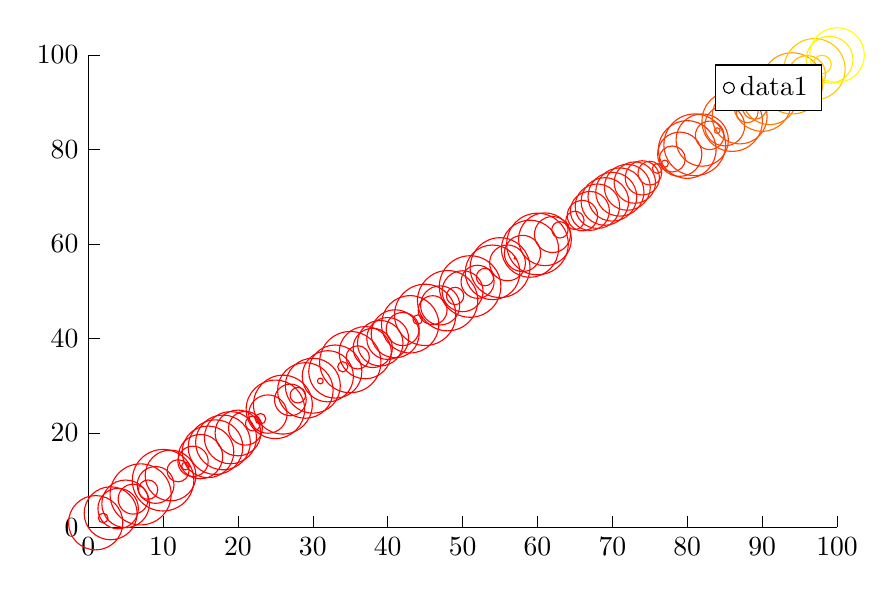
\begin{tikzpicture}

\begin{axis}[%
width=0.951\figureWidth,
height=\figureHeight,
at={(0\figureWidth,0\figureHeight)},
scale only axis,
colormap/redyellow,
every outer x axis line/.append style={black},
every x tick label/.append style={font=\color{black}},
every x tick/.append style={black},
xmin=   0,
xmax= 100,
every outer y axis line/.append style={black},
every y tick label/.append style={font=\color{black}},
every y tick/.append style={black},
ymin=   0,
ymax= 100,
axis background/.style={fill=white},
axis x line*=bottom,
axis y line*=left,
legend style={legend cell align=left, align=left, draw=black}
]
\addplot[scatter, only marks, mark=o, scatter src=explicit, scatter/use mapped color={mark options={}, draw=mapped color}, visualization depends on={\thisrow{size} \as \perpointmarksize}, scatter/@pre marker code/.append style={/tikz/mark size=\perpointmarksize}] table[row sep=crcr, meta=color]{%
x	y	size	color\\
   1	   1	9.81167	   1\\
   2	   2	1.7435	 256\\
   3	   3	9.5692	6561\\
   4	   4	7.30796	65536\\
   5	   5	8.60129	390625\\
   6	   6	5.41414	1.67962e+06\\
   7	   7	11.0291	5.7648e+06\\
   8	   8	3.49715	1.67772e+07\\
   9	   9	6.65142	4.30467e+07\\
  10	  10	11.1206	1e+08\\
  11	  11	9.17597	2.14359e+08\\
  12	  12	3.98306	4.29982e+08\\
  13	  13	1.40346	8.15731e+08\\
  14	  14	5.47687	1.47579e+09\\
  15	  15	8.00278	2.56289e+09\\
  16	  16	9.3269	4.29497e+09\\
  17	  17	9.87068	6.97576e+09\\
  18	  18	9.89277	1.102e+10\\
  19	  19	9.41976	1.69836e+10\\
  20	  20	8.26339	2.56e+10\\
  21	  21	6.10502	3.78229e+10\\
  22	  22	2.67611	5.48759e+10\\
  23	  23	1.93768	7.8311e+10\\
  24	  24	6.92784	1.10075e+11\\
  25	  25	10.5703	1.52588e+11\\
  26	  26	10.6343	2.08827e+11\\
  27	  27	5.72688	2.8243e+11\\
  28	  28	2.80514	3.77802e+11\\
  29	  29	10.0432	5.00246e+11\\
  30	  30	9.93248	6.561e+11\\
  31	  31	1.04329	8.52891e+11\\
  32	  32	9.24945	1.09951e+12\\
  33	  33	9.60379	1.40641e+12\\
  34	  34	1.84757	1.78579e+12\\
  35	  35	11.0691	2.25188e+12\\
  36	  36	4.19832	2.82111e+12\\
  37	  37	9.43543	3.51248e+12\\
  38	  38	7.08093	4.34779e+12\\
  39	  39	8.22117	5.35201e+12\\
  40	  40	7.56676	6.5536e+12\\
  41	  41	8.67349	7.98493e+12\\
  42	  42	5.97409	9.68265e+12\\
  43	  43	10.3546	1.16882e+13\\
  44	  44	1.69915	1.40482e+13\\
  45	  45	11.0738	1.68151e+13\\
  46	  46	5.20993	2.00476e+13\\
  47	  47	7.06604	2.38113e+13\\
  48	  48	10.8922	2.81793e+13\\
  49	  49	3.12412	3.32329e+13\\
  50	  50	7.39976	3.90625e+13\\
  51	  51	11.1176	4.57679e+13\\
  52	  52	5.97577	5.34597e+13\\
  53	  53	3.14382	6.22597e+13\\
  54	  54	9.87354	7.2302e+13\\
  55	  55	10.8101	8.37339e+13\\
  56	  56	6.46795	9.67173e+13\\
  57	  57	0.322121	1.11429e+14\\
  58	  58	6.54034	1.28063e+14\\
  59	  59	10.3016	1.4683e+14\\
  60	  60	11.1258	1.67962e+14\\
  61	  61	9.5407	1.91707e+14\\
  62	  62	6.50357	2.1834e+14\\
  63	  63	2.94855	2.48156e+14\\
  64	  64	0.444874	2.81475e+14\\
  65	  65	3.29985	3.18645e+14\\
  66	  66	5.48631	3.60041e+14\\
  67	  67	7.03046	4.06068e+14\\
  68	  68	8.03087	4.57163e+14\\
  69	  69	8.59718	5.13798e+14\\
  70	  70	8.81252	5.7648e+14\\
  71	  71	8.71447	6.45754e+14\\
  72	  72	8.2891	7.22204e+14\\
  73	  73	7.47524	8.0646e+14\\
  74	  74	6.17955	8.99195e+14\\
  75	  75	4.30552	1.00113e+15\\
  76	  76	1.80005	1.11303e+15\\
  77	  77	1.282	1.23574e+15\\
  78	  78	4.70419	1.37011e+15\\
  79	  79	7.98983	1.51711e+15\\
  80	  80	10.421	1.67772e+15\\
  81	  81	11.1487	1.85302e+15\\
  82	  82	9.45559	2.04414e+15\\
  83	  83	5.15215	2.25229e+15\\
  84	  84	1.01888	2.47876e+15\\
  85	  85	7.22268	2.72491e+15\\
  86	  86	10.9189	2.99218e+15\\
  87	  87	9.93985	3.28212e+15\\
  88	  88	3.96832	3.59635e+15\\
  89	  89	4.45188	3.93659e+15\\
  90	  90	10.5059	4.30467e+15\\
  91	  91	9.79797	4.70253e+15\\
  92	  92	1.97155	5.13219e+15\\
  93	  93	7.64389	5.59582e+15\\
  94	  94	11.0532	6.09569e+15\\
  95	  95	4.47898	6.6342e+15\\
  96	  96	6.62228	7.2139e+15\\
  97	  97	11.0589	7.83743e+15\\
  98	  98	3.3127	8.50763e+15\\
  99	  99	8.46952	9.22745e+15\\
 100	 100	9.88174	1e+16\\
};
\addlegendentry{data1}

\end{axis}
\end{tikzpicture}%
\end{document}